%
% Documento: Fundamentação Teórica
%

\chapter{HTML}
\label{chap:HTML}
\section{Revendo os conceitos}
HTML é a linguagem principal para criação de documentos, e aplicações, na \textit{Web}, para o uso de todos, em qualquer lugar \cite{W3Chtml2015}.

O documento HTML consiste em uma árvore de elementos e texto. Cada elemento é representado por uma \textit{tag} de abertura e uma de fechamento. As \textit{tags} têm de estar todas aninhadas completamente, sem haver sobreposição. Os elementos podem ter atributos que controlam o comportamento do elemento \cite{HTMLspec2014}.

Os navegadores \textit{web} (\textit{Browsers}) traduzem esse formato em uma árvore DOM (\textit{Document Object Model}). Uma árvore DOM é uma representação em memória de um documento, que possui vários nós, cada nó agrupando alguns atributos do documento.

\begin{figure}[!htb]
	\centering
	\caption{Exemplo de estrutura da árvore do DOM}
	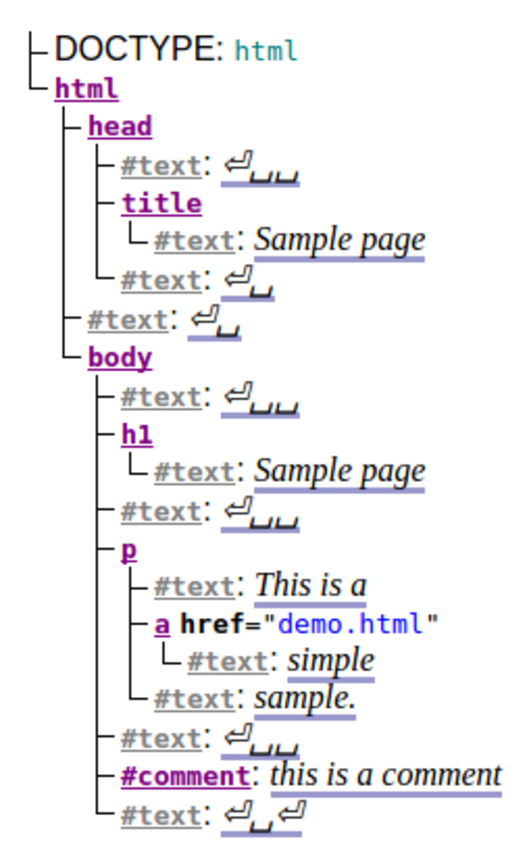
\includegraphics[width=0.3\textwidth]{./04-figuras/DOMsnippet}
	\fonte{\citeonline{HTMLspec2014}}
	\label{fig:domtree}
\end{figure}

Na figura \autoref{fig:domtree} vê-se que o elemento raiz da árvore é o html, já que este é o tipo do documento interpretado. Cada elemento do html é representado por um nó, todos os elementos que se encontram no nível abaixo deste são denominados descendentes (\textit{descendant}), os nós que se encontram exatamente um nível abaixo são os filhos (\textit{child}), e os elementos que se encontram no mesmo nível são chamados de irmãos (\textit{sinbling}). Os nós demonidados de text são os nós que encapsulam os textos inseridos dentro dos elementos html, então estes serão os nós que existiram em maior número no DOM.

\chapter{CSS}
\label{chap:CSS}
\section{Revendo os conceitos}

CSS é um mecanismo simples para adicionar estilo (\textit{e.g.}, fontes, cores, espaçamento) em documentos \textit{Web} \cite{W3Ccss2015}.

Uma folha de estilo \(C\) pode ser vista como um conjunto de regras \(R\), composto por regras simples \(R_i\), cada uma composta por um seletor \(S_i\) e um conjunto de pares: propriedade \(P_i\) e seus valores \(V_i\). Os seletores definem a quais elementos de um documento, serão aplicadas as propriedades definidas pela regra à qual elas pertencem \cite{Geneves2012}.

\subsection{Seletores}
\label{subsec:seletores}
Um seletor é uma cadeia de uma, ou mais, sequências de seletores simples, separados por combinadores. Os seletores simples são cadeias de caracteres que representam um elemento do html: o seletor universal, representado pelo simbolo \(\ast\), indica que a regra será aplicada a todos os elementos que estejam no DOM. O seletor de elementos html, representado pelo nome da \textit{tag} de um elemento, por exemplo \(h1\). O seletor de classe, que seleciona todos os elementos que possuam o atributo \(class\) especificado pelo seletor, é utilizado escrevendo-se o nome da classe, precedido pelo simbolo \(\#\). O seletor de \(id\), seleciona o elemento do html que possua aquele \(id\), é utilizado escrevendo-se o identificador precedido de um ponto final (\(.\)). 
Simplificando, sem perder generalidade, podemos considerar que regras são feitas de seletores únicos que definem uma única propriedade por vez. Os seletores \(S_i\), chamados de padrões na especificação do CSS \cite{CSSspec2009}, definem uma função booleana na forma:
\begin{equation}
	expression * element \rightarrow boolean
\end{equation}
que define se um elemento é, ou não, selecionado pela expressão do seletor.

Os combinadores são propriedades que definem relações entre os elementos de um documento. Existem três formas de combinadores: descendentes, filhos e irmãos. O combinador de descendente descreve qualquer elemento que esteja um nível abaixo na árvore DOM, e são representados pelo espaço em branco, \textit{e.g.} "$body\ p$". O combinador de filho descreve os elementos que estão exatamente um nível abaixo do nó, este combinador é representado pelo sinal de maior ($>$), \textit{e.g.} "$body > p$". O combinador de irmãos descreve os elementos que estão no mesmo nível da árvore, existem duas variações, uma para o próximo irmão adjacente ($+$) e um para todos os irmãos ($\tilde{~}$).

\subsection{Efeito Cascata}
\label{subsec:cascade}

O efeito cascata do CSS se dá devido à ordem de precedência dos valores de propriedades definidas para cada elemento. O mecanismo recebe uma lista desordenada destas propriedades, e as organiza pela precedência das declarações delas. Essa ordem é definida de acordo com os critérios listados abaixo, em ordem decrescente de prioridade \cite{CSScascade2015}.

\begin{itemize}
	\item \textbf{Origem e Importância:} 
	Cada regra de estilo possui uma origem, que define onde ela estará na cascada, e a importância se refere à utilização, ou não, do atributo $!important$.
	\item \textbf{Escopo:}
	Uma declaração pode ter uma subárvore do DOM como escopo, afetando somente os elementos pertencentes a esta subárvore. Para declarações normais, o escopo mais interno tem prioridade, para regras com $!important$ as regras do escopo mais externo sobrescreverá.
	\item \textbf{Especificidade:}
	O calculo de especificidade conta a ocorrência de seletores de ID, classe e tipo (\textit{tags} e \textit{pseudo-elements}), e faz-se uma soma ponderada dessas ocorrências. A declaração com maior especificidade tem prioridade.
	\item \textbf{Ordem de aparição:}
	A última declaração no documento tem a maior prioridade. Isto significa que a localidade será levada em conta, para isso, considera-se que as folhas de estilo são concatenadas ao documento na ordem em que são declaradas.
\end{itemize}

